\documentclass{article}

%\usepackage{haldefs}
\usepackage{url}
\usepackage{graphicx}
\usepackage[margin=1in]{geometry}
\usepackage{parskip}
\usepackage[normalem]{ulem}
\usepackage{subcaption}
\usepackage{float}

\title{Project 4}

\author{Maks Cegielski-Johnson\\u0836524}
% IF YOU'RE USING THIS .TEX FILE AS A TEMPLATE, PLEASE REPLACE
% The author WITH YOUR NAME AND UID.
% Replace the due date with anyone you worked with i.e. "Worked with: John McCarthy, Watson, & Hal-9000"

\begin{document}

\maketitle


\section{Getting Started}

\textbf{What type of personal data would you like to visualize?}

Daily calorie intake

\textbf{How do you obtain the data?}

Manually collected by looking at the nutritional information and Google queries. This could have also been done in conjunction with a calorie counting application, which would help by storing the data as well as providing easier calorie lookup tools.

\textbf{Why studying such a data set is important and meaningful for you?}

In order to try to maintain a healthy lifestyle, I am interested in seeing if there is a better way to count calories than pen/paper or using an application. 

\textbf{What sort of insights do you expect to get out of this visualization?}

I want to determine if the use of physical visualization can make a larger impact on one's desire to count calories than a non-physical visualization. 

\section{Design Process}

\textbf{What sort of physical medium/building block do you choose to use? And why do you choose such	a material?}

I chose to use marbles and a two small cardboard boxes. I needed some sort of token to represent a quantity of calories, and I wanted this token to be tactilely pleasing. My thought was that ideally, this visualization would have some aesthetic element, so that it could be both be placed anywhere in one's household for use, as well as to invoke some calming emotion rather than being visually aggressive (such as using colorful lego blocks). 

\textbf{What sort of computation/data analysis do you have to do prior to creating your physical visualization?}

Since this is a very basic mapping between data and token, the only computation required is to convert calories into units of 50 kCal (with each marble representing 50 kCal). Since this visualization is meant to only provide a rough guideline/idea of how many calories one is intaking, rounding of calories is fine to either overcount or slightly undercount. 

\textbf{How do you evaluate the effectiveness of your physical visualization?}

Because this isn't an HCI class, I didn't perform any formal verification (i.e studies or interviews) to determine the effectiveness of the visualization, and instead all analysis was done by me to see if the visualization was effective for me personally. 

If I wanted to formally check effectiveness, I would have given this visualization to a few friends who have a history of counting calories, and asked them to use the tool for a few weeks and maintain a journal, concluding with an interview to gather more information. 



\section{Creating the Physical Visualization}

\textbf{After you have completed the physical visualization, what sort of insights do you end up obtaining from the visualization?}

Personally, I found it both more impactful and more motivating to use the marbles rather than paper/pen or an app. Seeing how many calories different foods have made a big impact of what I should and should not be eating. Being able to hold the amount of calories I had left in my day had more of an impact than seeing some number of equal amount. 

If I wanted to eat some snack, I could see exactly what fraction of a meal this snack was equivalent to, and how I could eat something healthier and more filling with the same or less calories. 

\textbf{Describe the encoding you used for your physical visualization and how would a viewer interpret it.}

Two storage containers (source and sink) and $k$ marbles, each equivalent to 50 calories. If your diet is $N$ calories per day, then place $k = \lfloor N/50\rfloor$ in one container (for example 30 marbles if you want to eat 1500 calories per day).

After consuming some $m$ calories, move $round(m/50)$ marbles from the source container to the sink container. Greedily rounding up will result in eating less calories than alloted, and rounding down will result in slight overeating. Best judgement should be used to edge cases. 

A user can eye-ball roughly how many calories they have ate and have left, as well as explicitly count the marbles. 

Given proper marbles and/or containers, this visualization can be extended to:

\begin{itemize}
\item Add marbles to the source if some exercise is performed to burn calories.
\item Have a sink container with multiple chambers, for example, 3 chambers for breakfast, lunch, and dinner. Marbles would be placed accordingly and each meal can be visualized seperately. This could also be done with having 3 different colored sets of marbles. 
\end{itemize} 

\pagebreak

\section{Images}

\begin{figure}[H]
	\centering
	\begin{subfigure}{.5\textwidth}
		\centering
		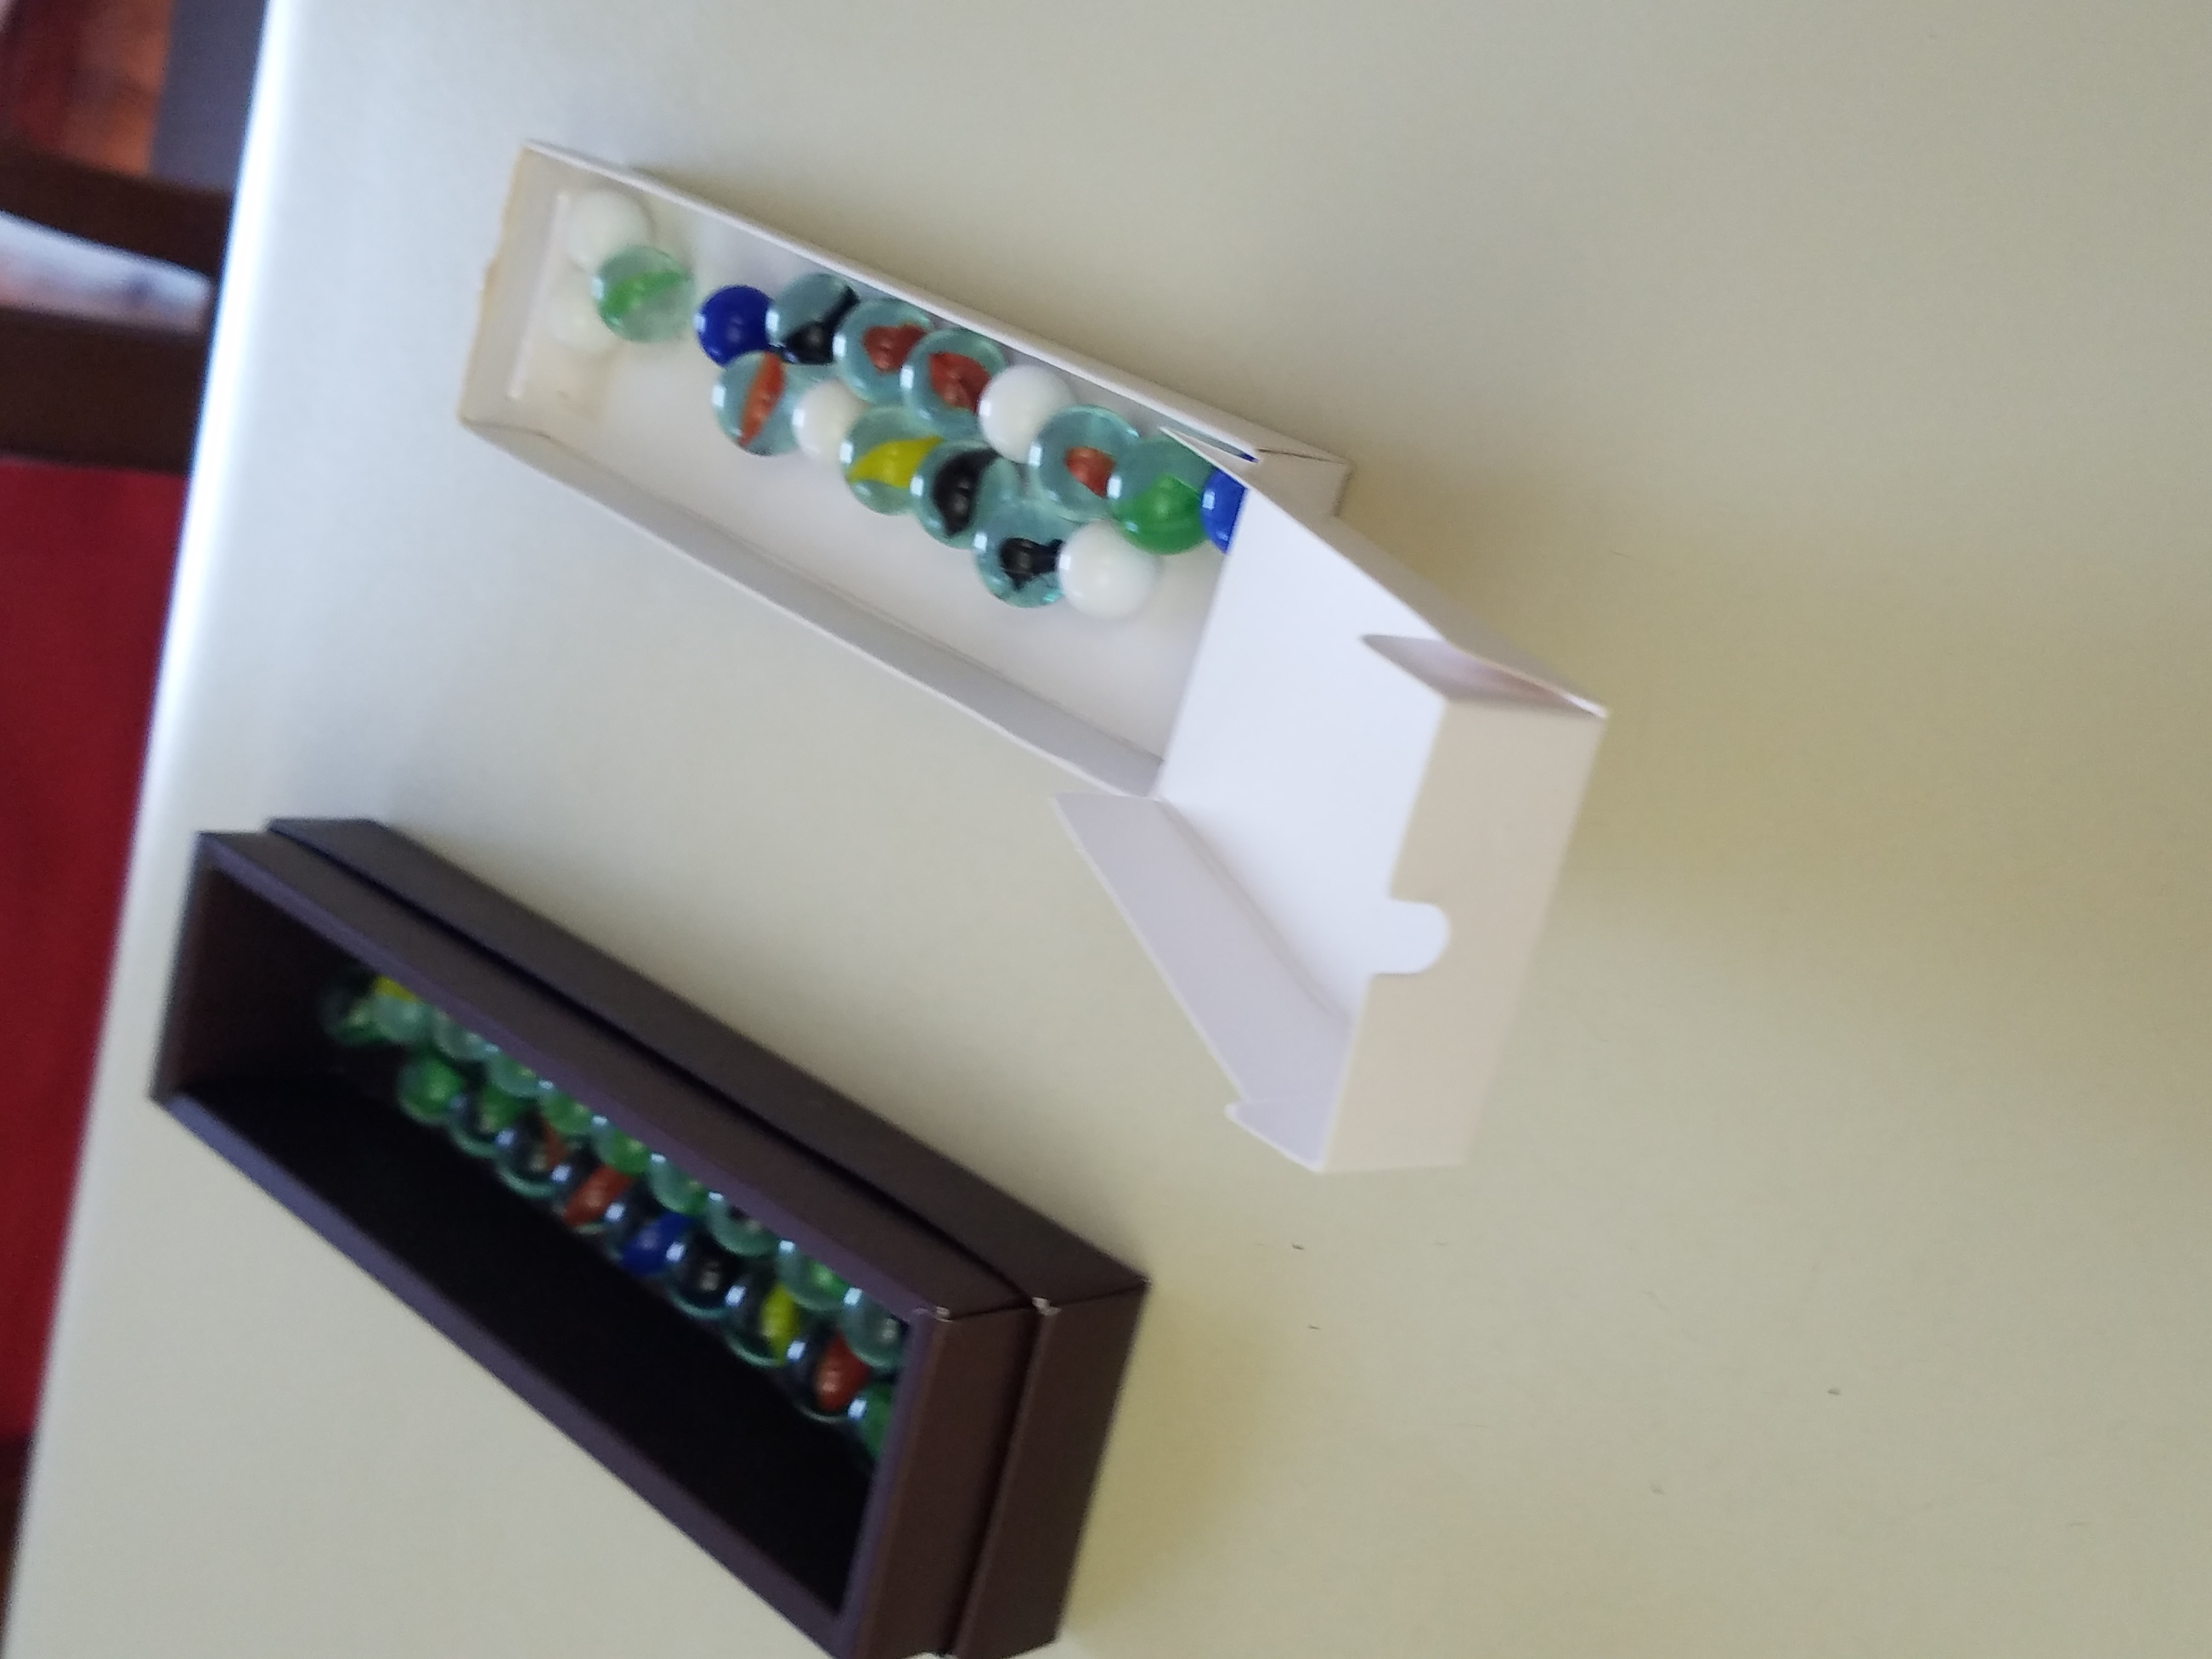
\includegraphics[width=.9\linewidth,angle=-90]{photos/m1}
	\end{subfigure}%
	\begin{subfigure}{.5\textwidth}
		\centering
		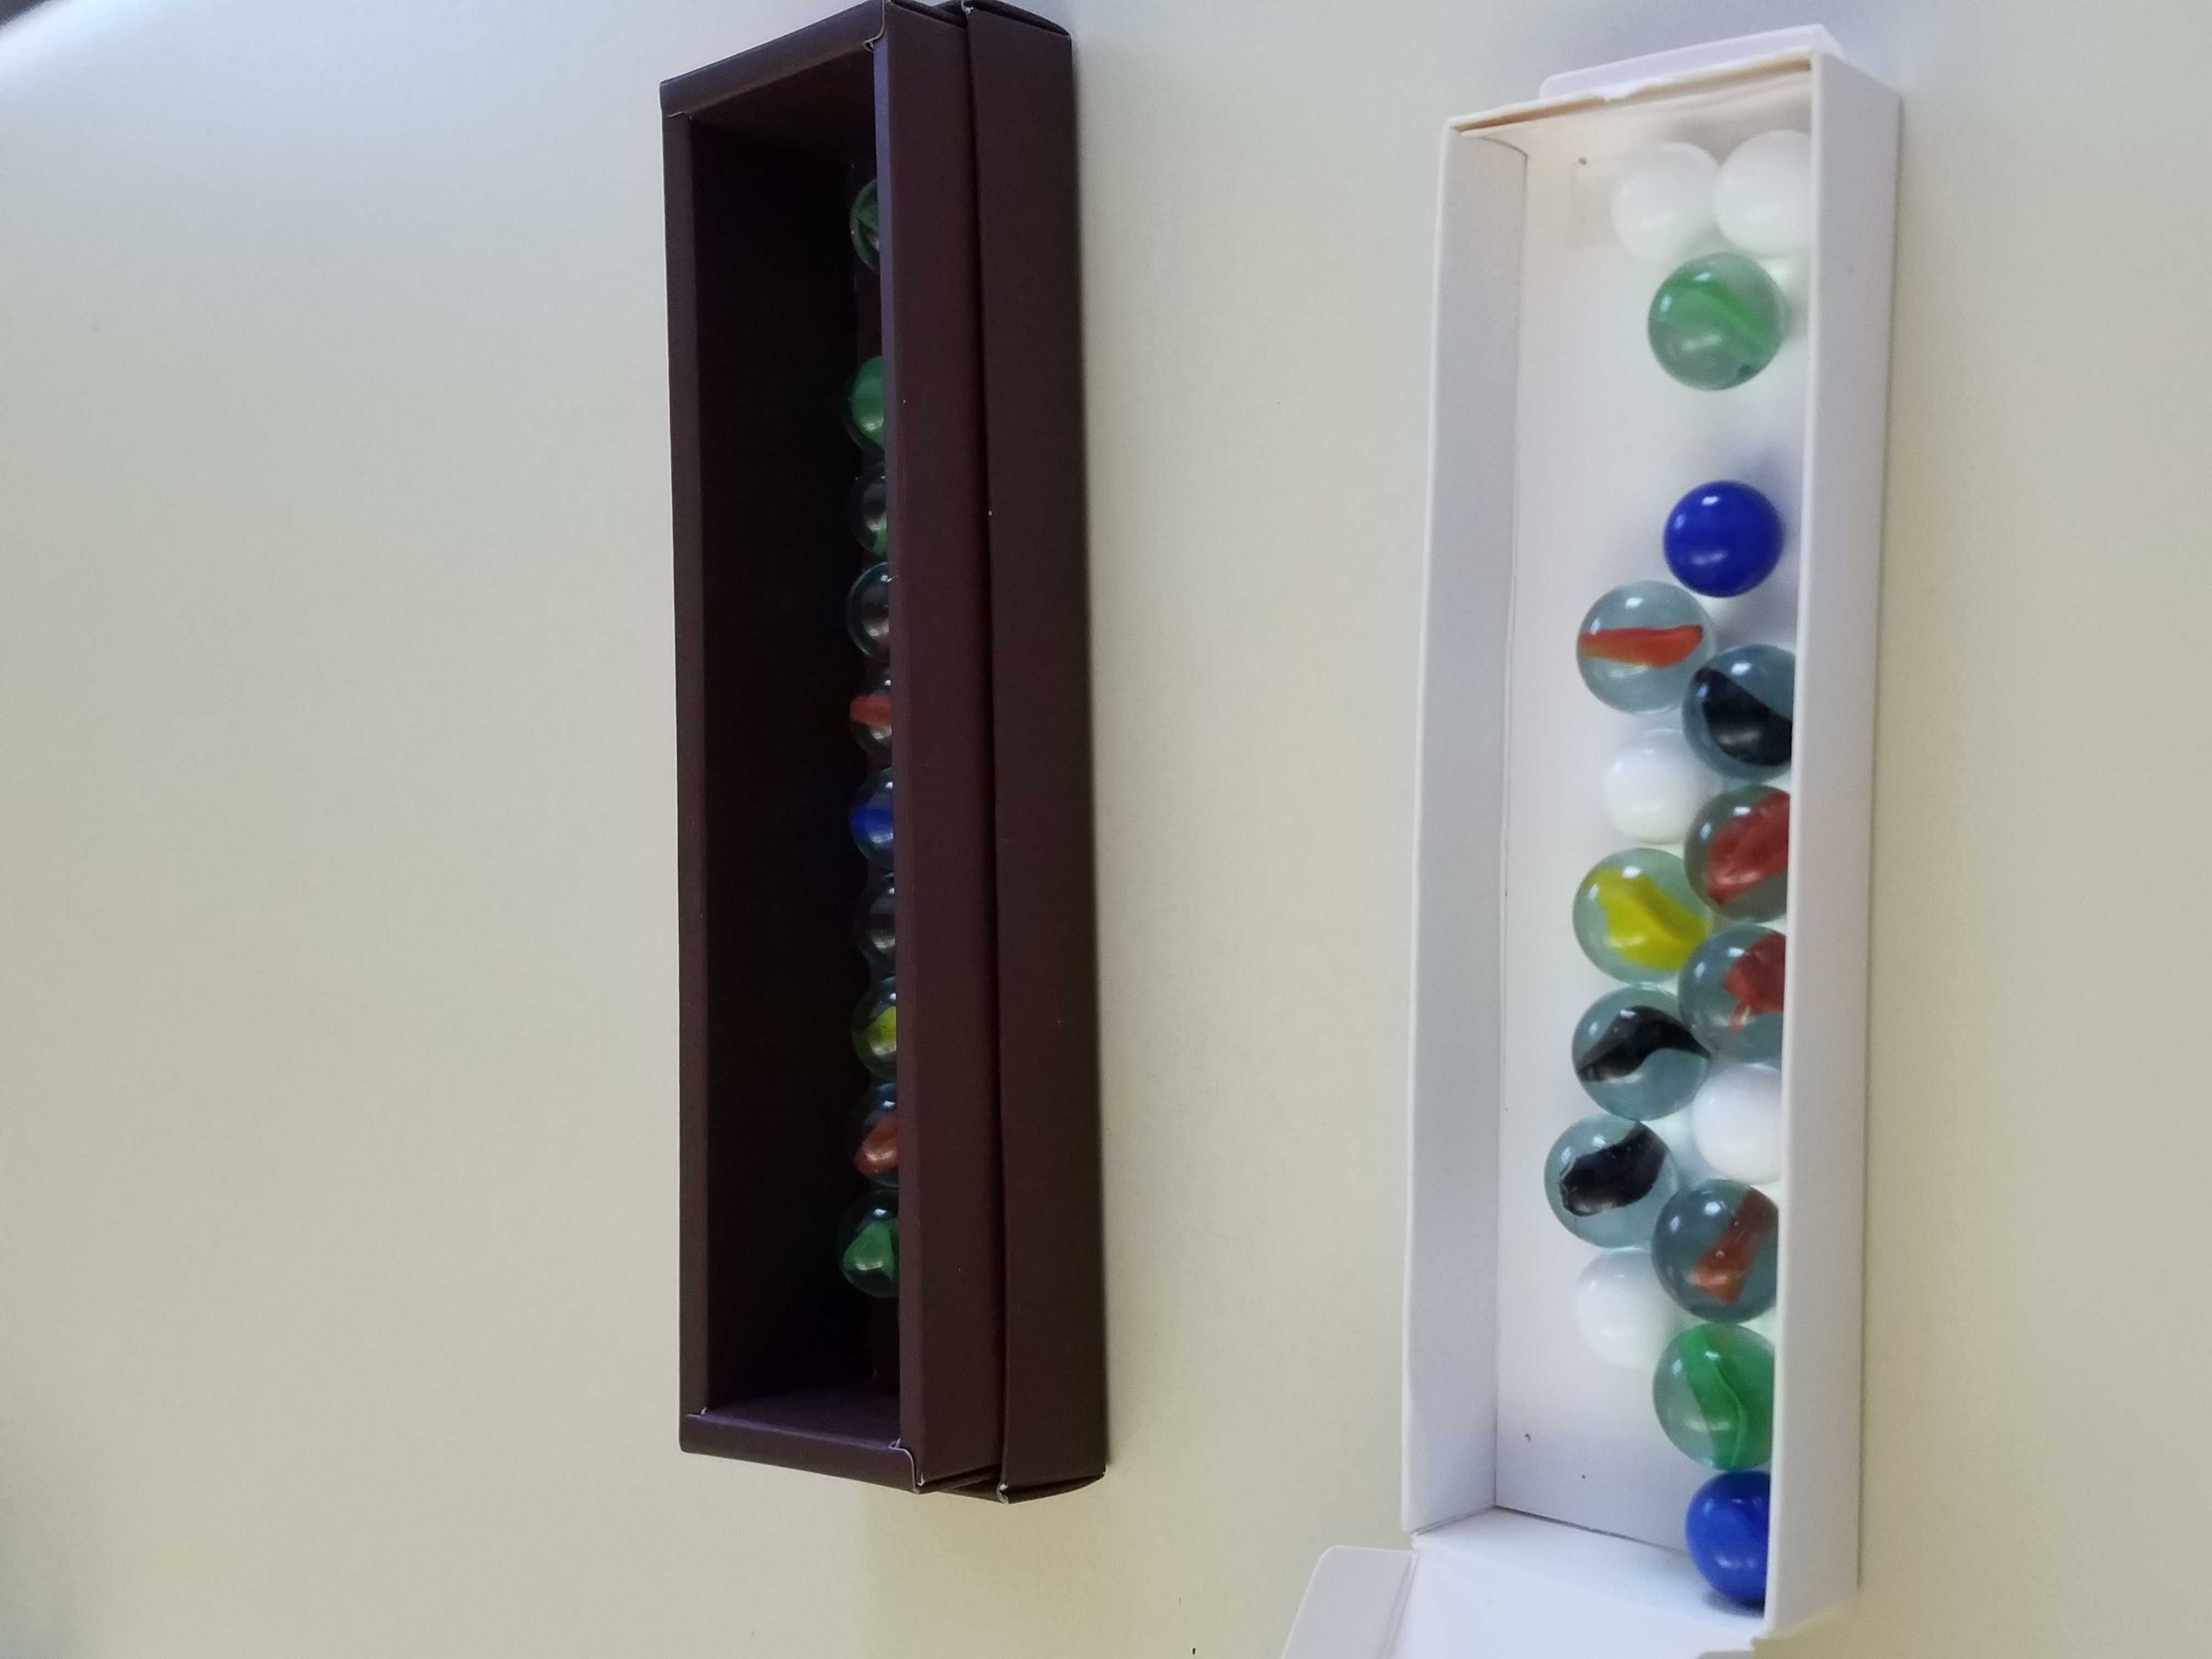
\includegraphics[width=.9\linewidth,angle=-90]{photos/m2}
	\end{subfigure}
\end{figure}

\begin{figure}[H]
	\centering
	\begin{subfigure}{.5\textwidth}
		\centering
		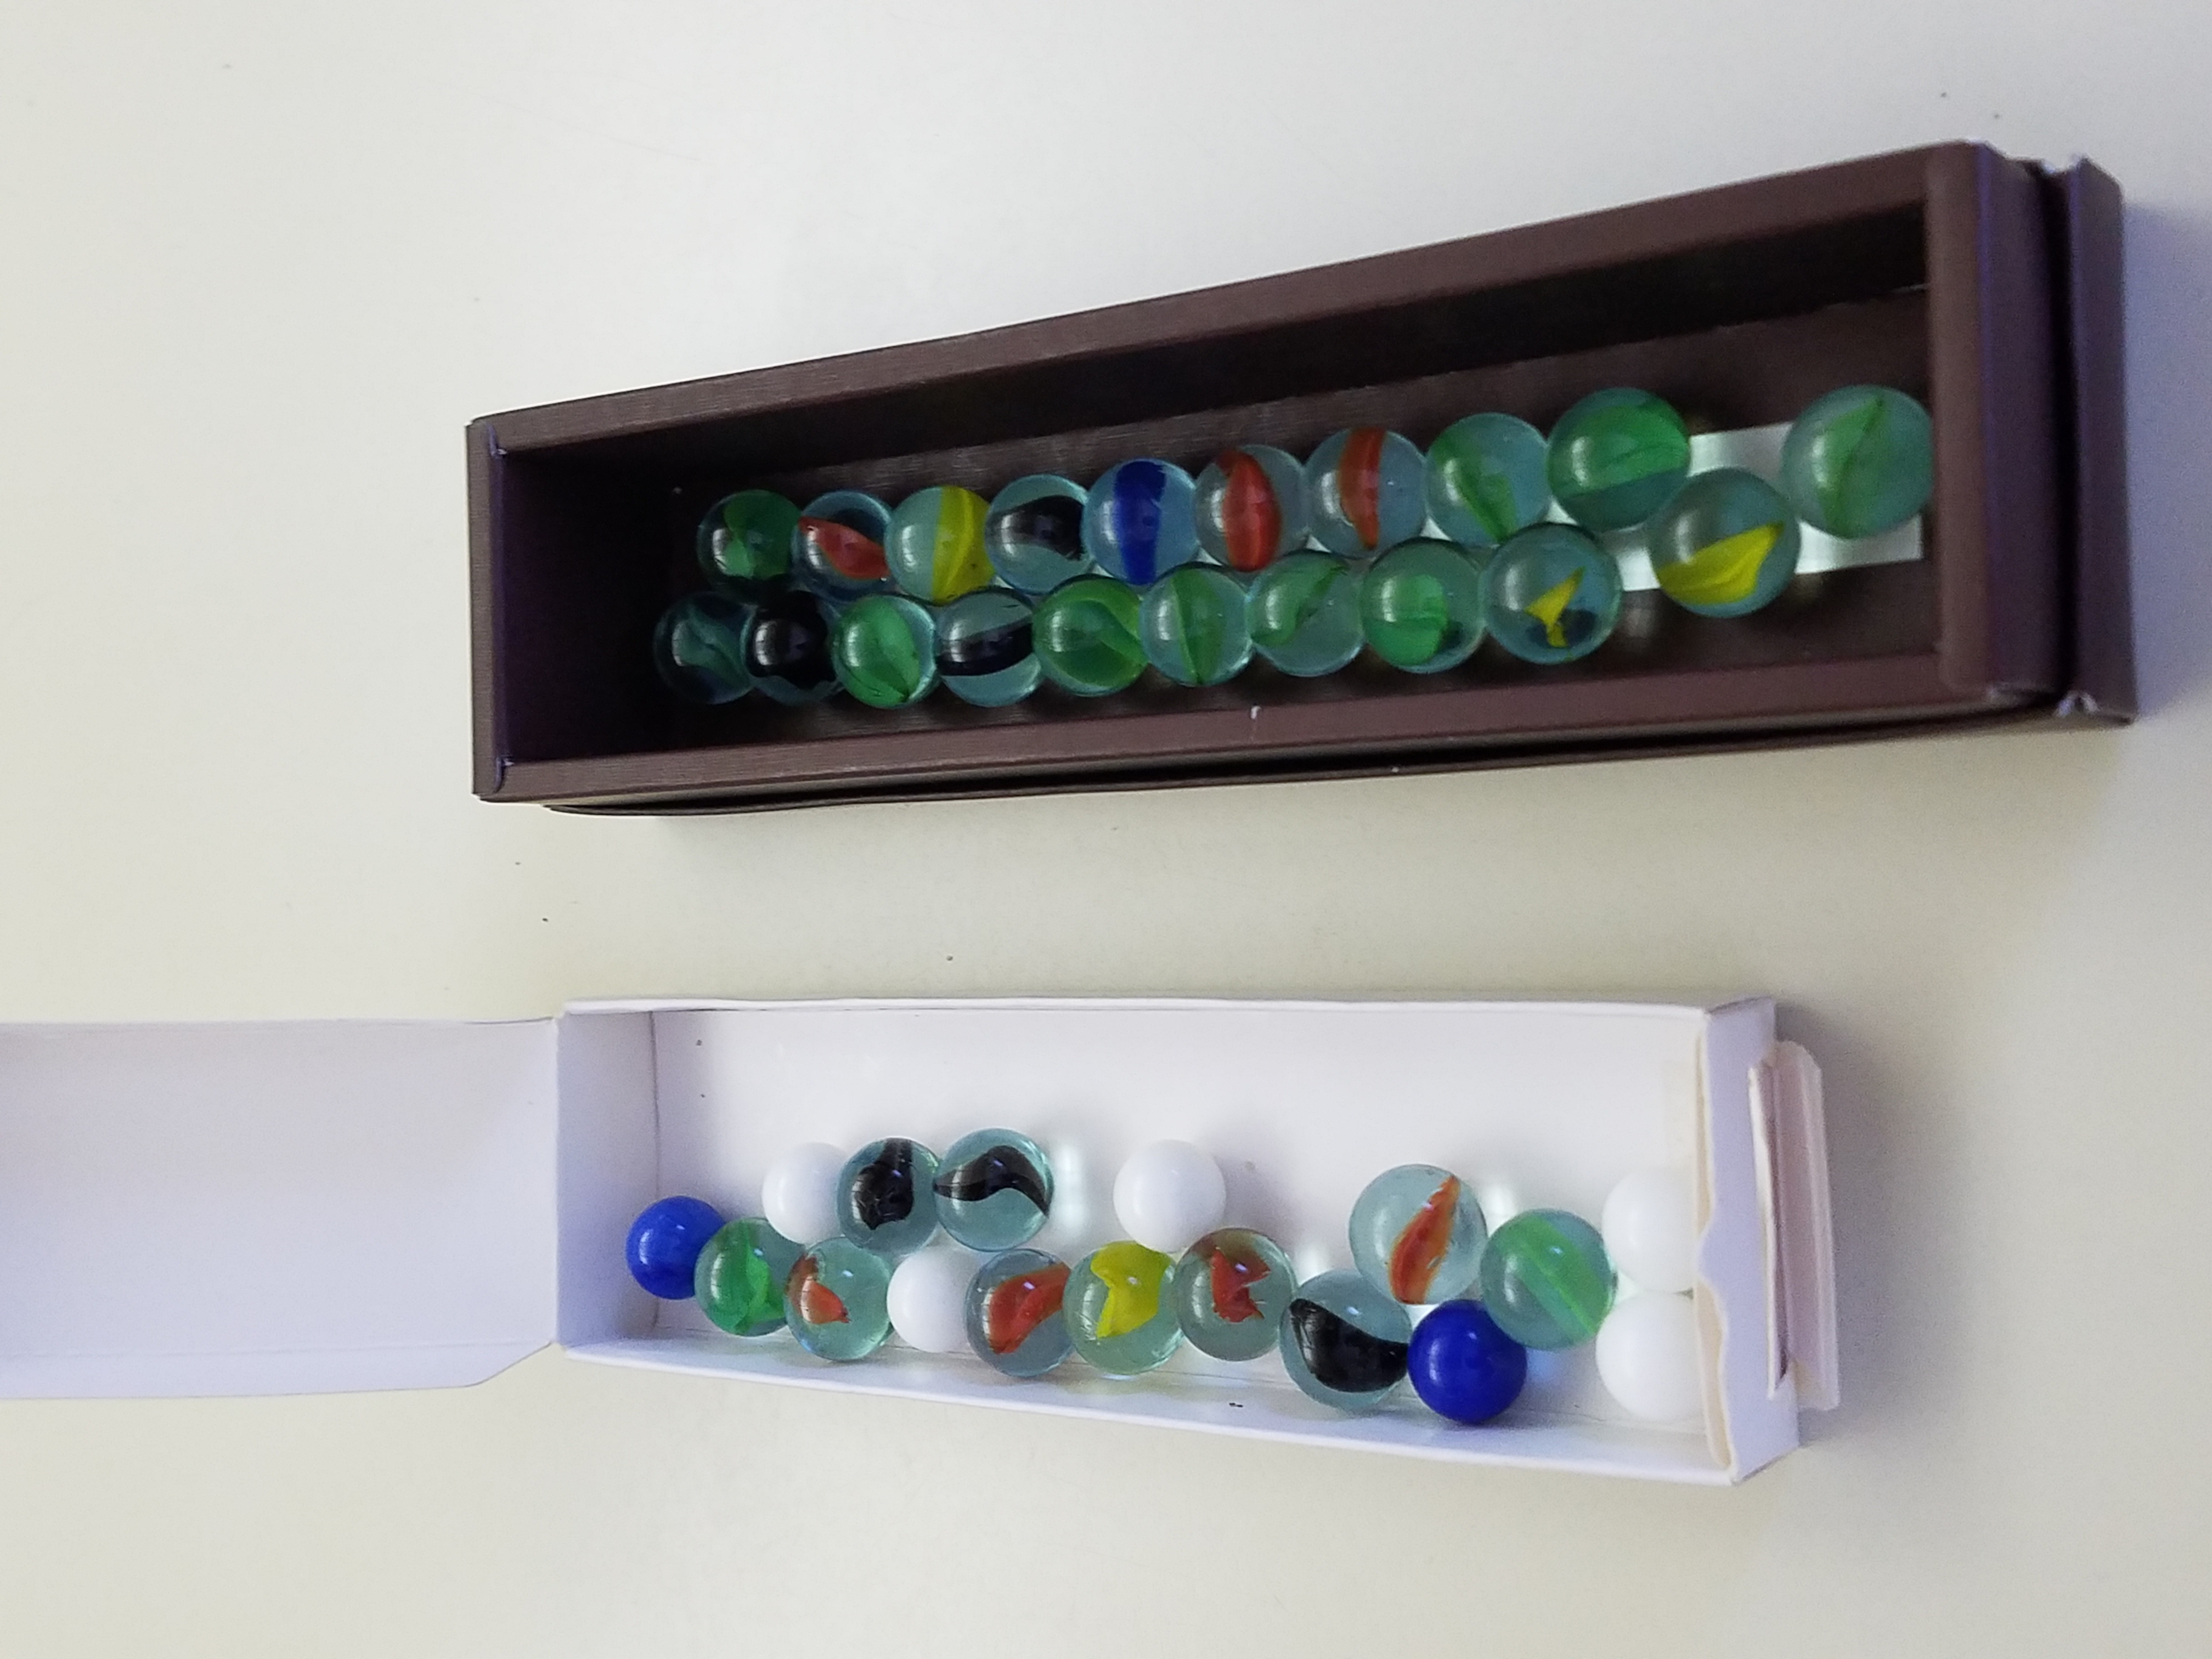
\includegraphics[width=.9\linewidth,angle=-90]{photos/m3}
	\end{subfigure}%
	\begin{subfigure}{.5\textwidth}
		\centering
		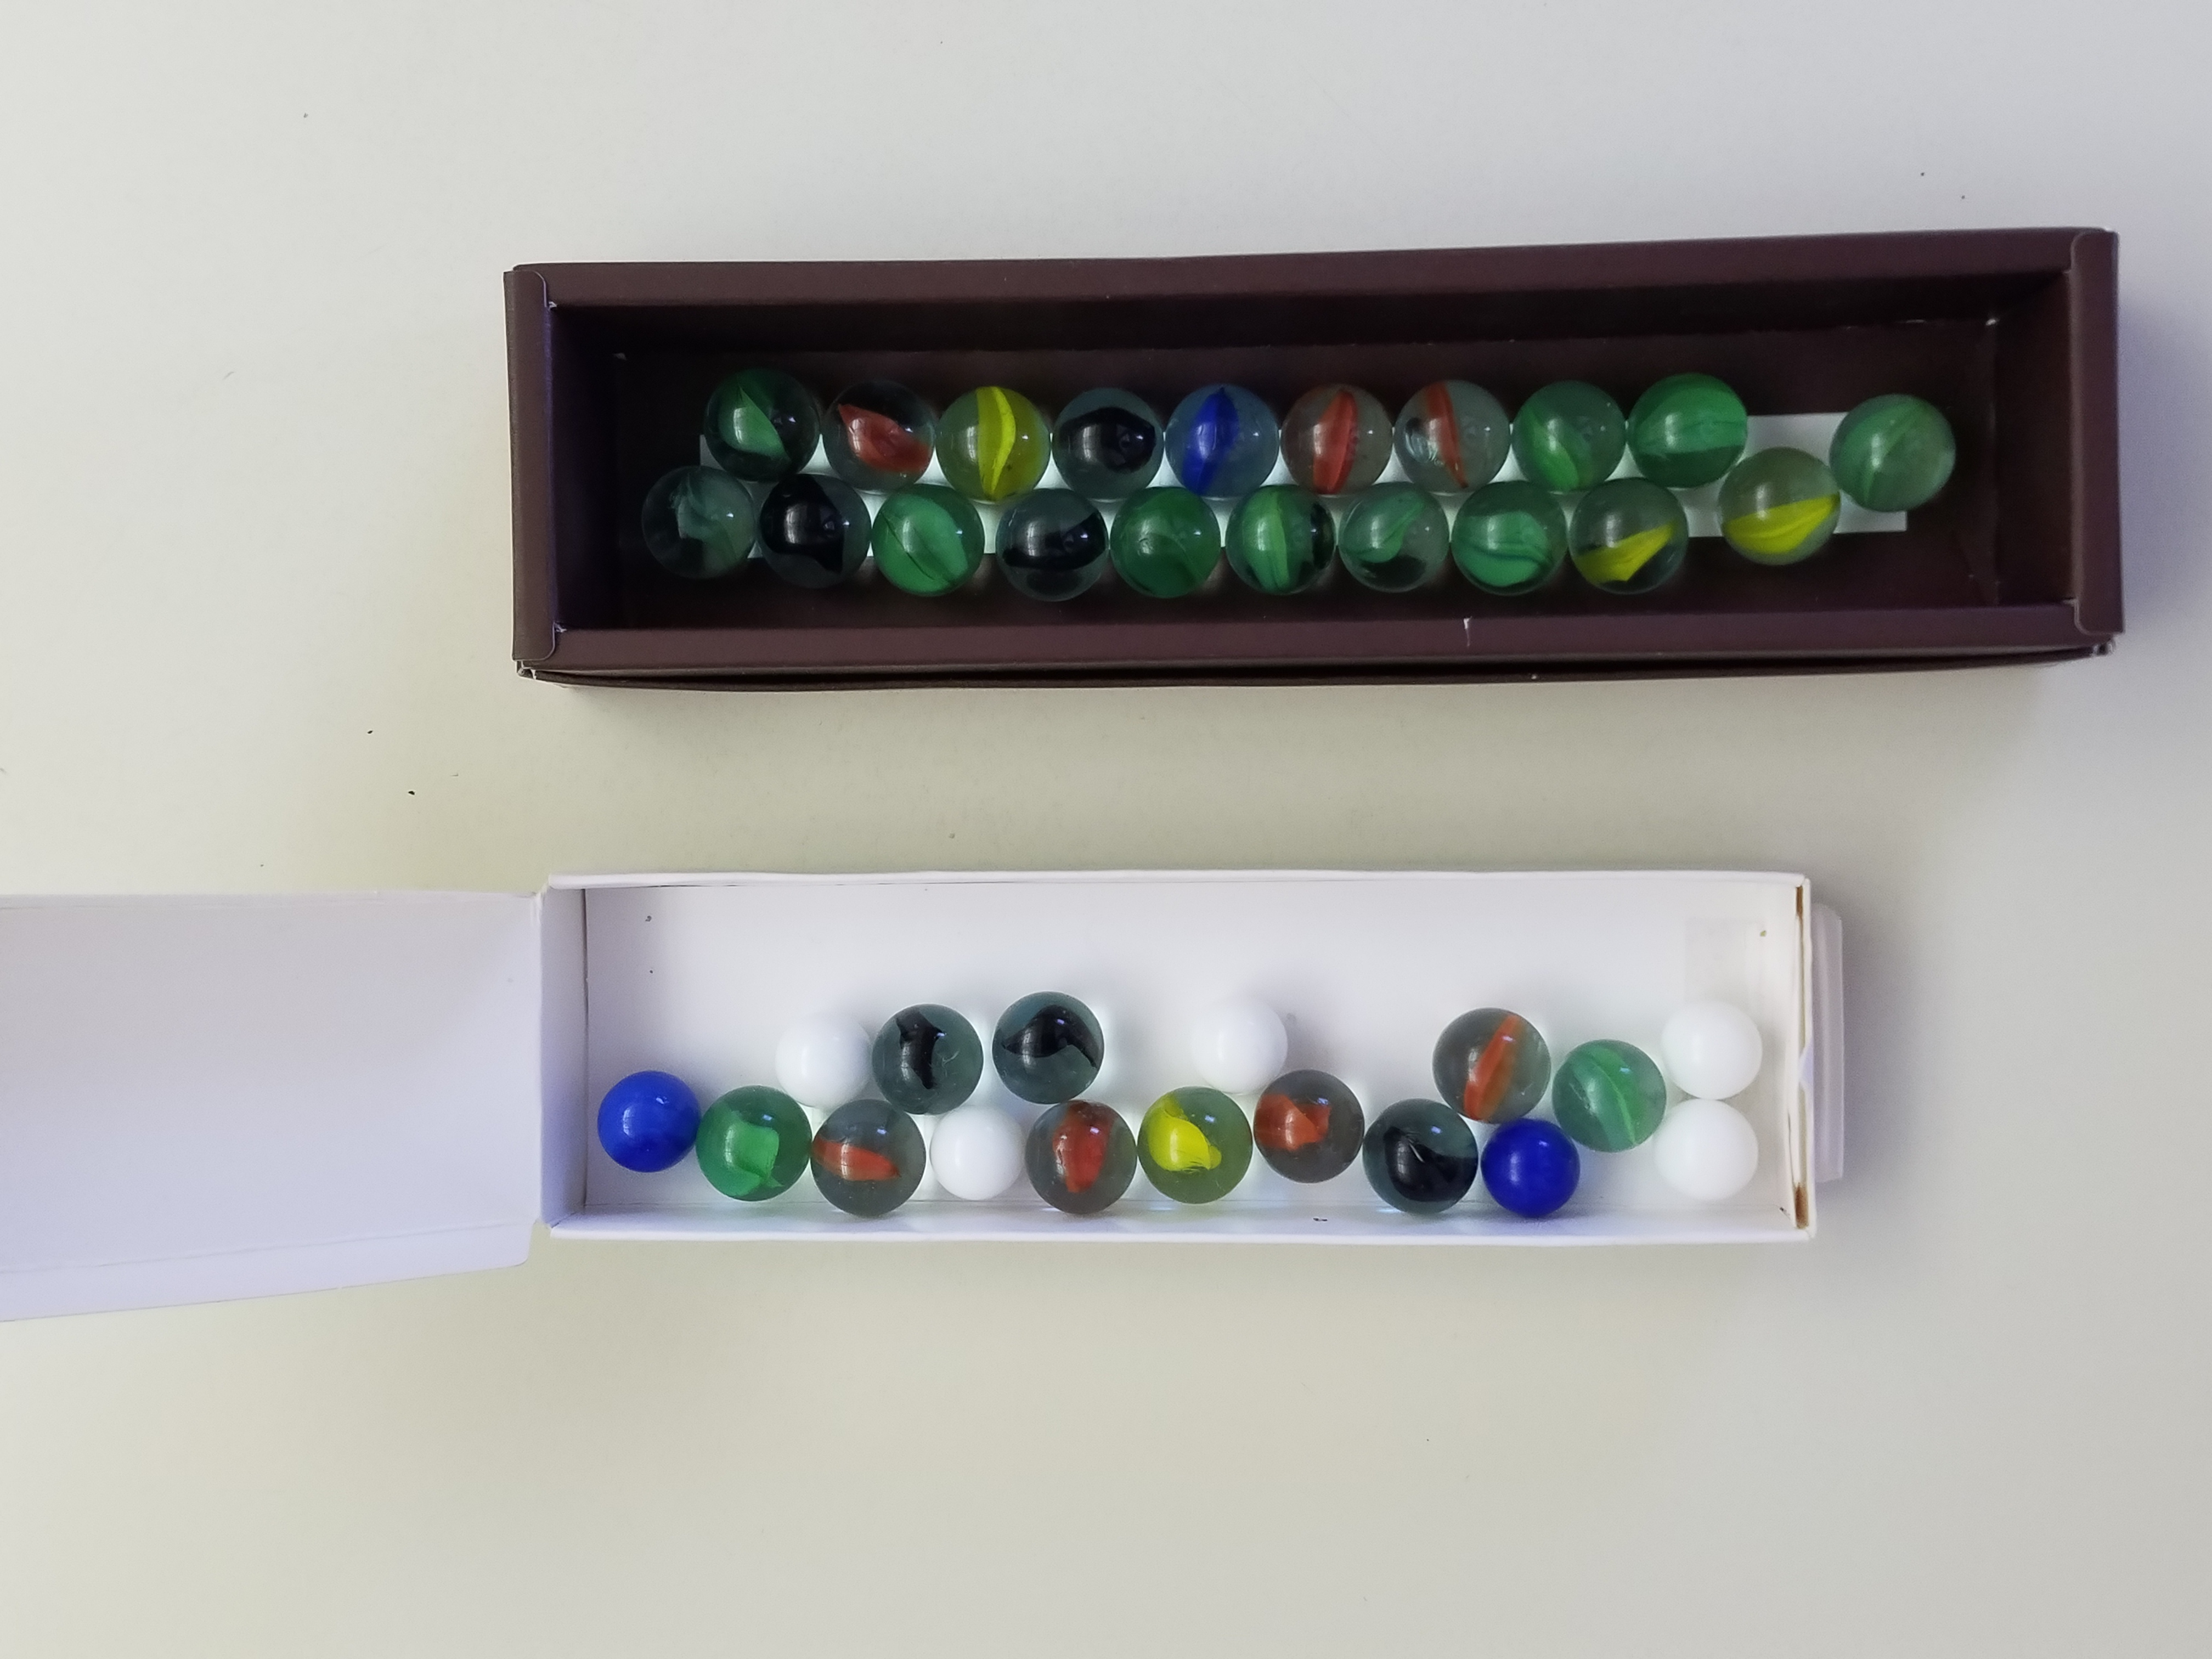
\includegraphics[width=.9\linewidth,angle=-90]{photos/m4}
	\end{subfigure}
\end{figure}




\end{document}
